\documentclass{beamer}
\usepackage[utf8]{inputenc}
\usepackage[english,russian]{babel}
\usetheme{Madrid}
\usepackage{graphicx}
\graphicspath{{imgs/}}

\title{Разработка ПО для онлайн монитора светимости детектора Belle II}
\author{Каня К. О. \\
        Научный руководитель: Ремнев М. А.}
\institute{Новосибирский Государственный Университет}



\makeatletter

\setbeamertemplate{footline}
{
  \leavevmode%
  \hbox{%
  %\begin{beamercolorbox}[wd=.333333\paperwidth,ht=2.25ex,dp=1ex,center]{author in head/foot}%
  %  \usebeamerfont{author in head/foot}Каня Кирилл, НГУ
  %\end{beamercolorbox}%
  \begin{beamercolorbox}[wd=.5\paperwidth,ht=2.25ex,dp=1ex,left]{title in head/foot}%
    \usebeamerfont{title in head/foot} kania.kirill@gmail.com
  \end{beamercolorbox}%
  \begin{beamercolorbox}[wd=.5\paperwidth,ht=2.25ex,dp=1ex,right]{date in head/foot}%
    \usebeamerfont{date in head/foot}\insertshortdate{}\hspace*{2em}
    \insertframenumber{} / \inserttotalframenumber\hspace*{2ex} 
  \end{beamercolorbox}}%
  \vskip0pt%
}
\makeatother


\begin{document}

\begin{frame}
\titlepage
\end{frame}

\begin{frame}
\frametitle{Belle II}
    \begin{itemize}
        \item superKEKB $e^+e^-$ коллайдер ($E_{e^-}=7$ГэВ, $E_{e^+}=4$ГэВ)
        \item Проектная светимость $8\cdot10^{35}$\text{с}$^{-1}$\text{см}$^{-2}$
        \item Изучение редких распадов B- и D-мезонов
        \item Поиск новой физики
    \end{itemize}
    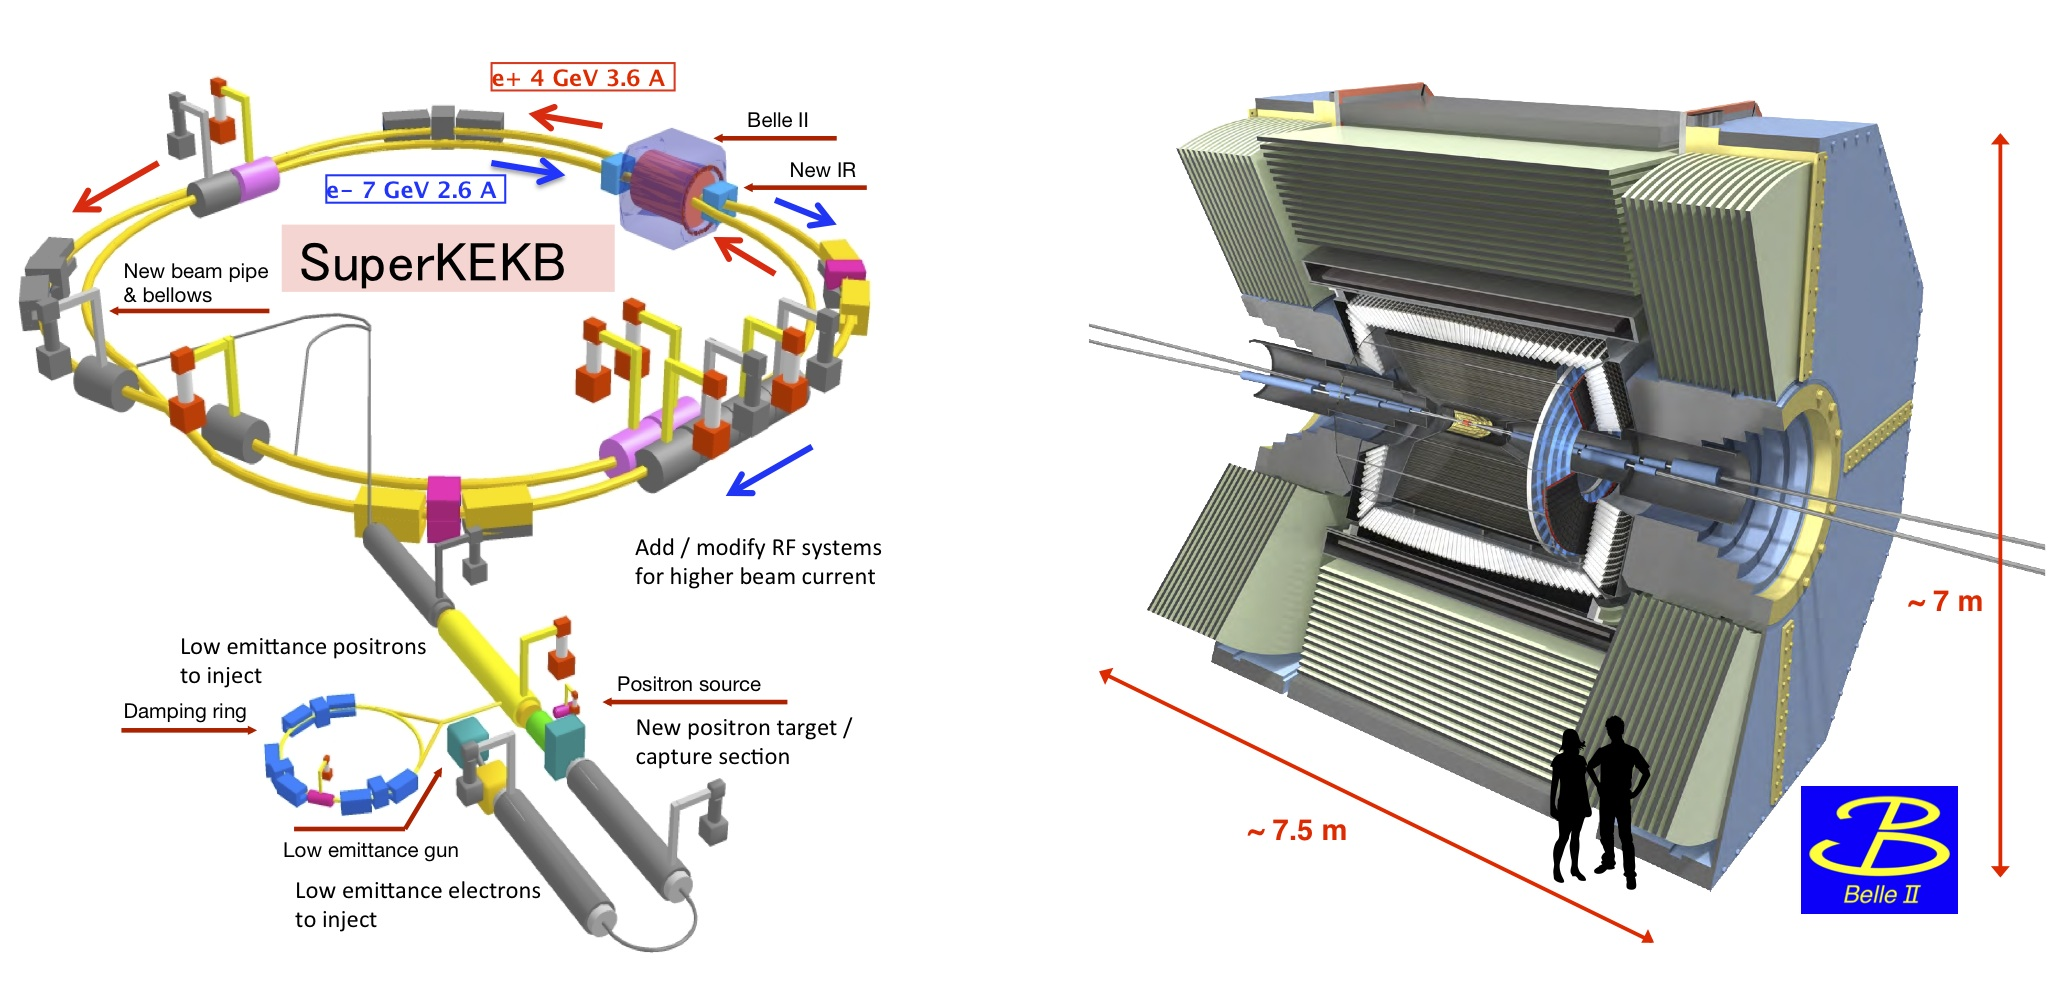
\includegraphics[width=\textwidth]{SuperKEKB_BelleII.jpg}
\end{frame}

\begin{frame}
\frametitle{Электромагнитный калориметр ECL}
    \begin{columns}
        \begin{column}{0.5\textwidth}
            \begin{itemize}
                \item 8736 \textit{CsI} кристаллов
                \item Регистрация фотонов и электронов
                \item 20 МэВ - 8 ГэВ
                \item Светимость онлайн/офлайн
            \end{itemize}
        \end{column}
        \begin{column}{0.5\textwidth}
            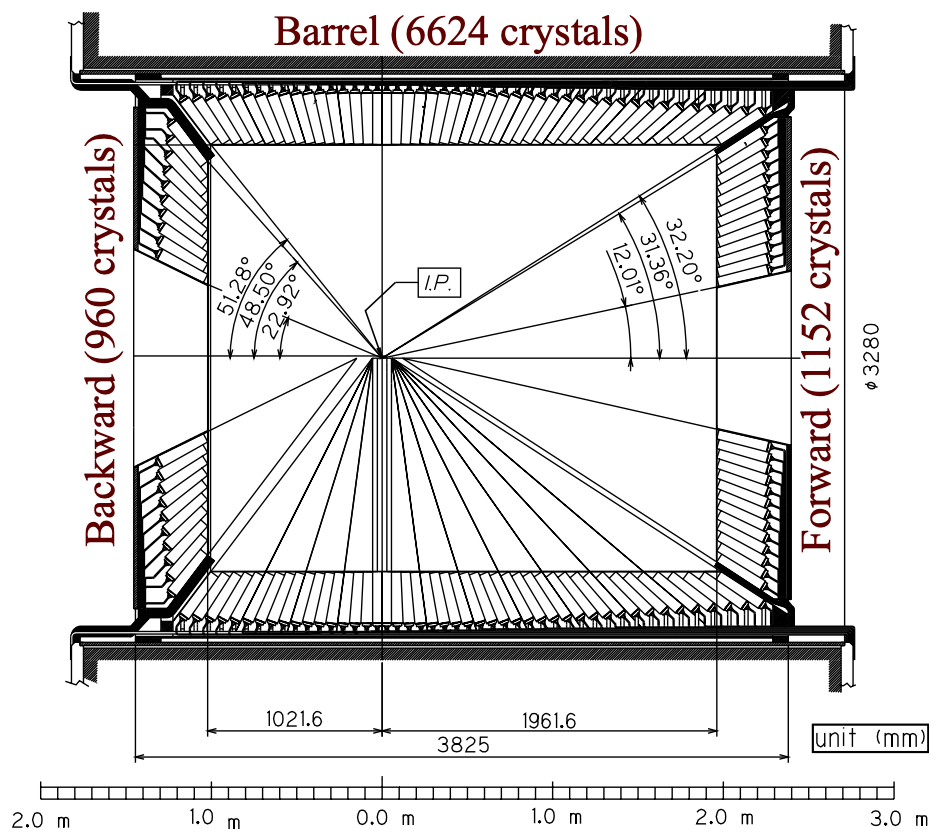
\includegraphics[width=\textwidth]{ECL}
        \end{column}
    \end{columns}
\end{frame}

\begin{frame}
\frametitle{Онлайн монитор светимости (LOM)}
Разработан в институте ядерной физики
    \begin{itemize}
        \item Измеряет скорость счета $e^+e^-$ рассеяния с ECL
        \item Контроль процесса набора данных
        \item Отслеживание работы ускорителя
    \end{itemize}
    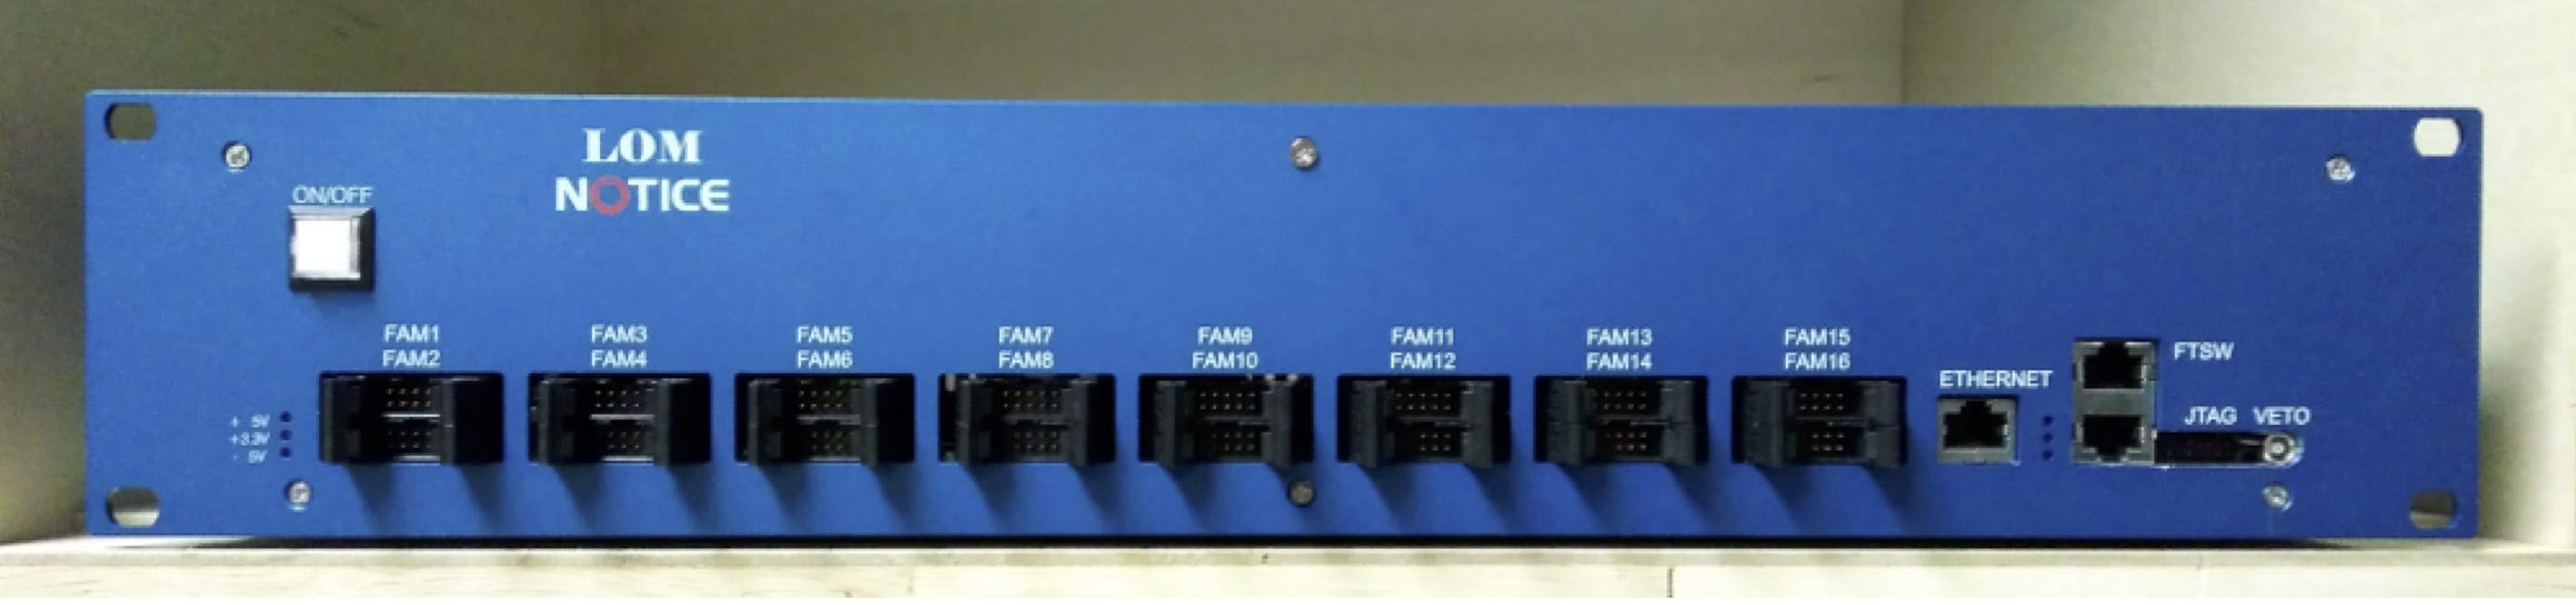
\includegraphics[width=\textwidth]{LOM_picture}
\end{frame}


%переписать
\begin{frame}
\frametitle{Задачи}
Разработать ПО которое обеспечит:
  \begin{itemize}
    \item Первичную проверку качества
    \item Архивирование данных
    \item Отображение данных
    \item Передачу данных
    \item Отказоустойчивость
  \end{itemize}
\end{frame}

% Убрать картинку со старой версией ПО, добавить картинку с диаграмой считывающего данные софта
\begin{frame}
\frametitle{Архитектура ПО}
    \begin{itemize}
        \item Python 2.7 + библиотека pythonIOC (EPICS PV)
        \item ПО было существенно расширено и оптимизировано 
        \\~\\
    \end{itemize}
%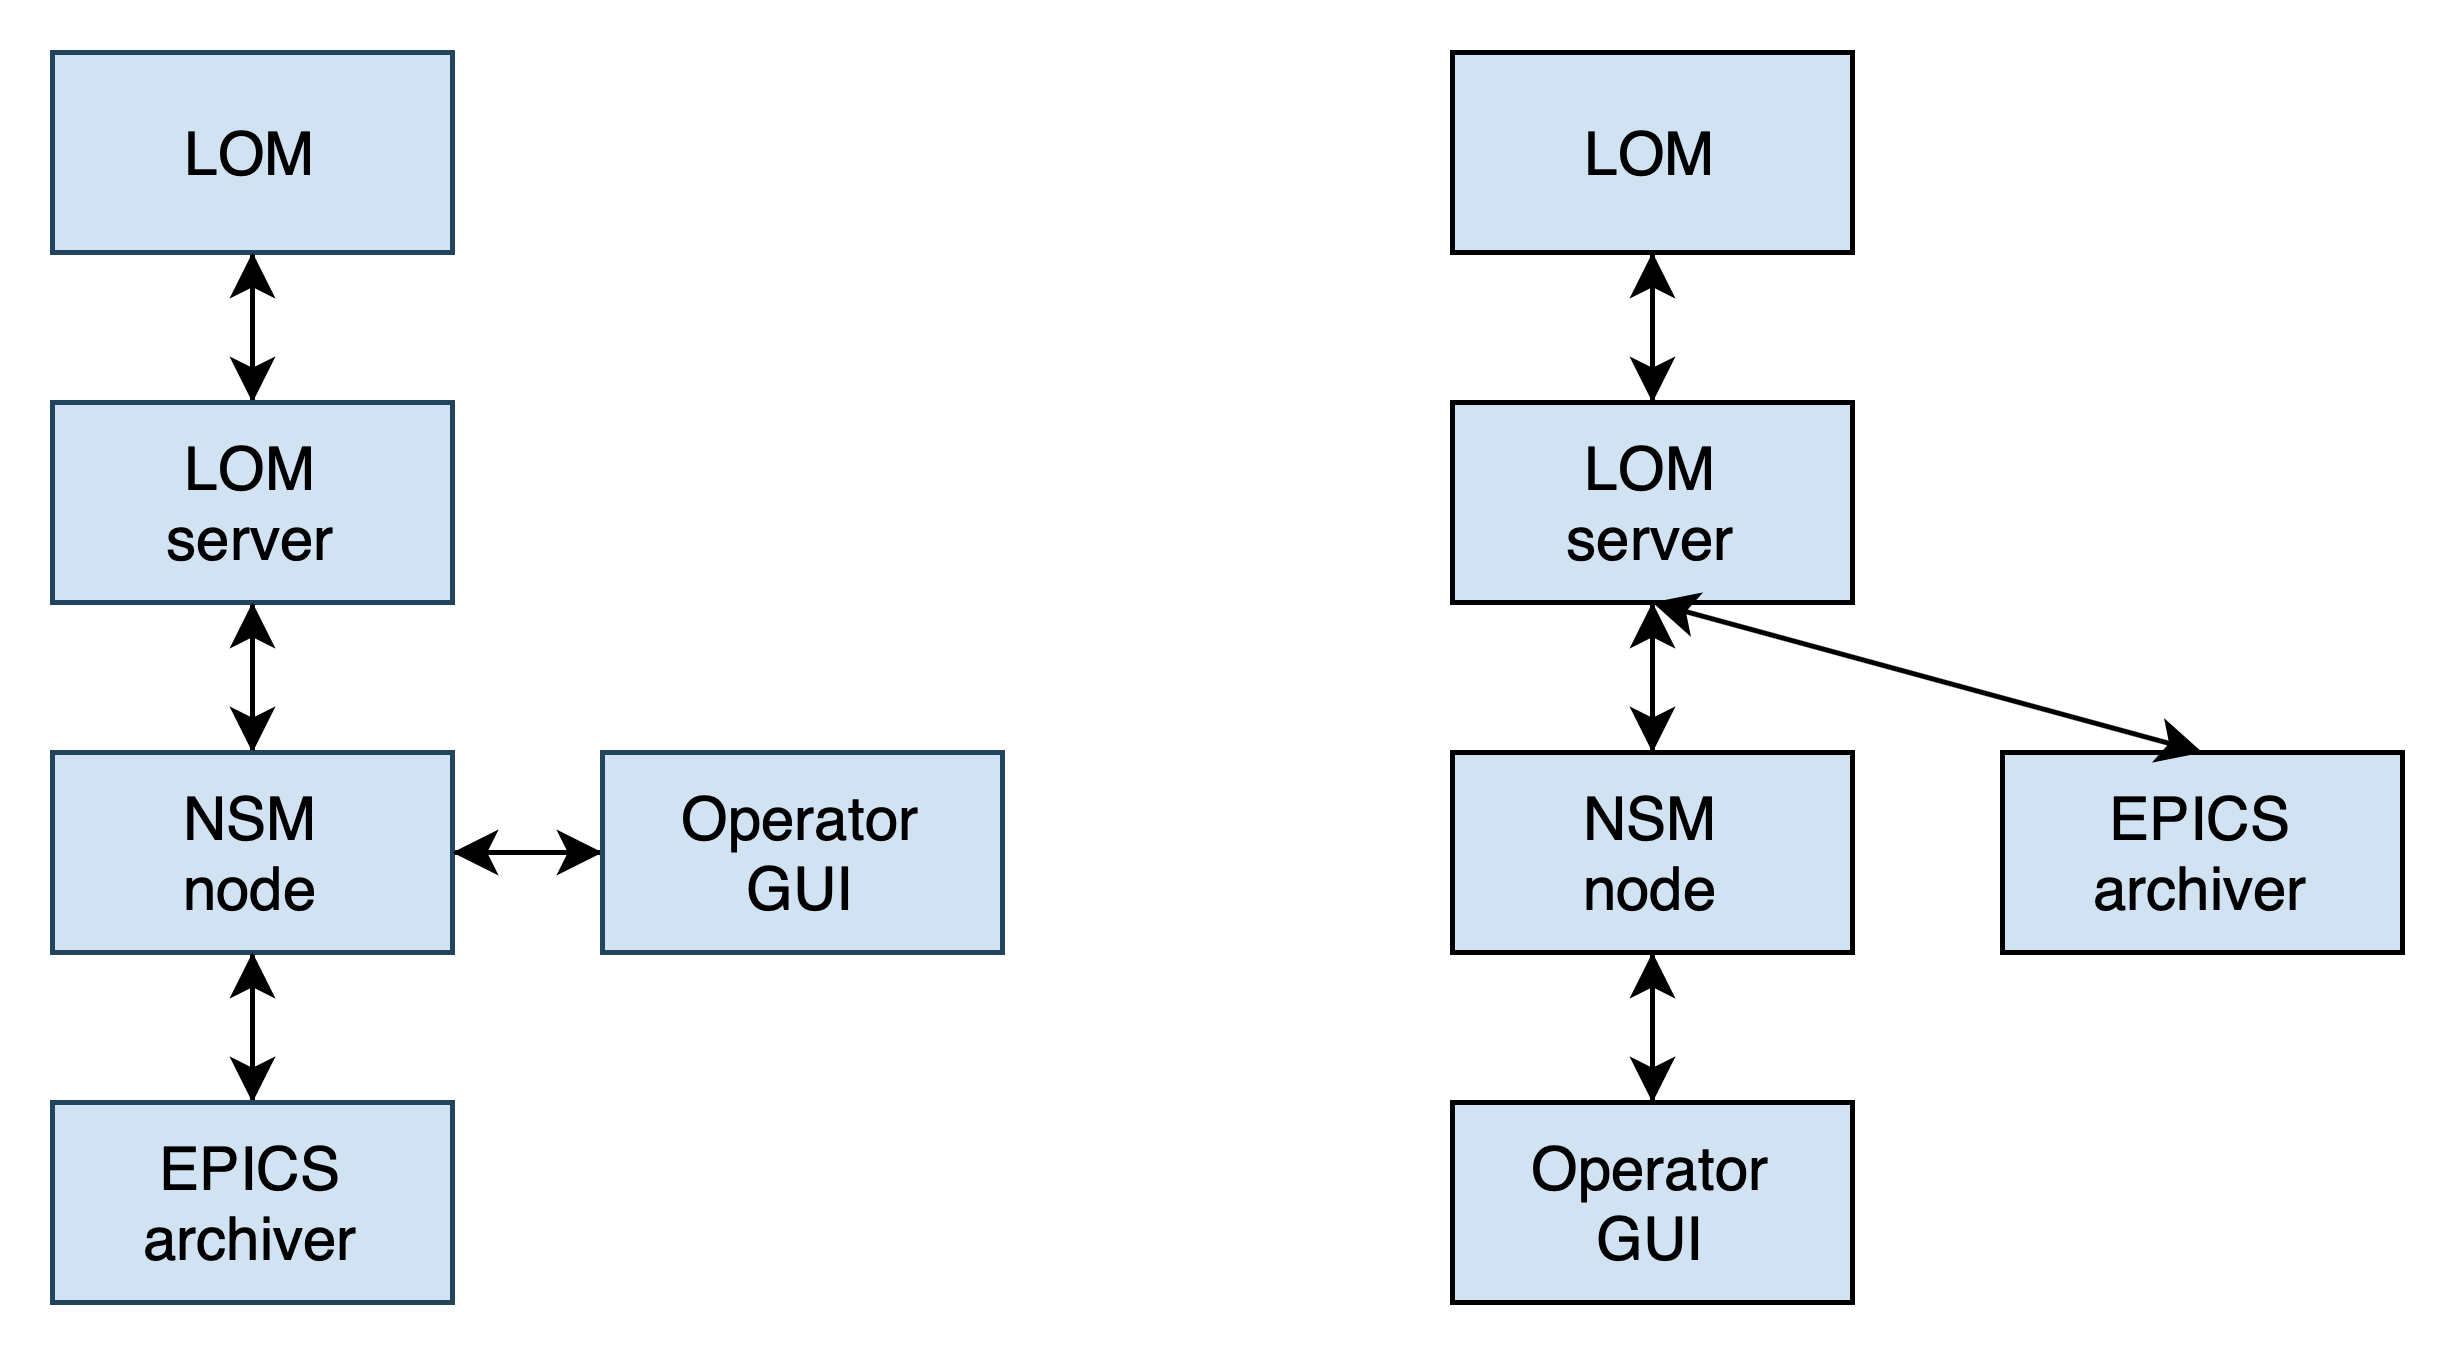
\includegraphics[width=\textwidth]{Architecture.png}
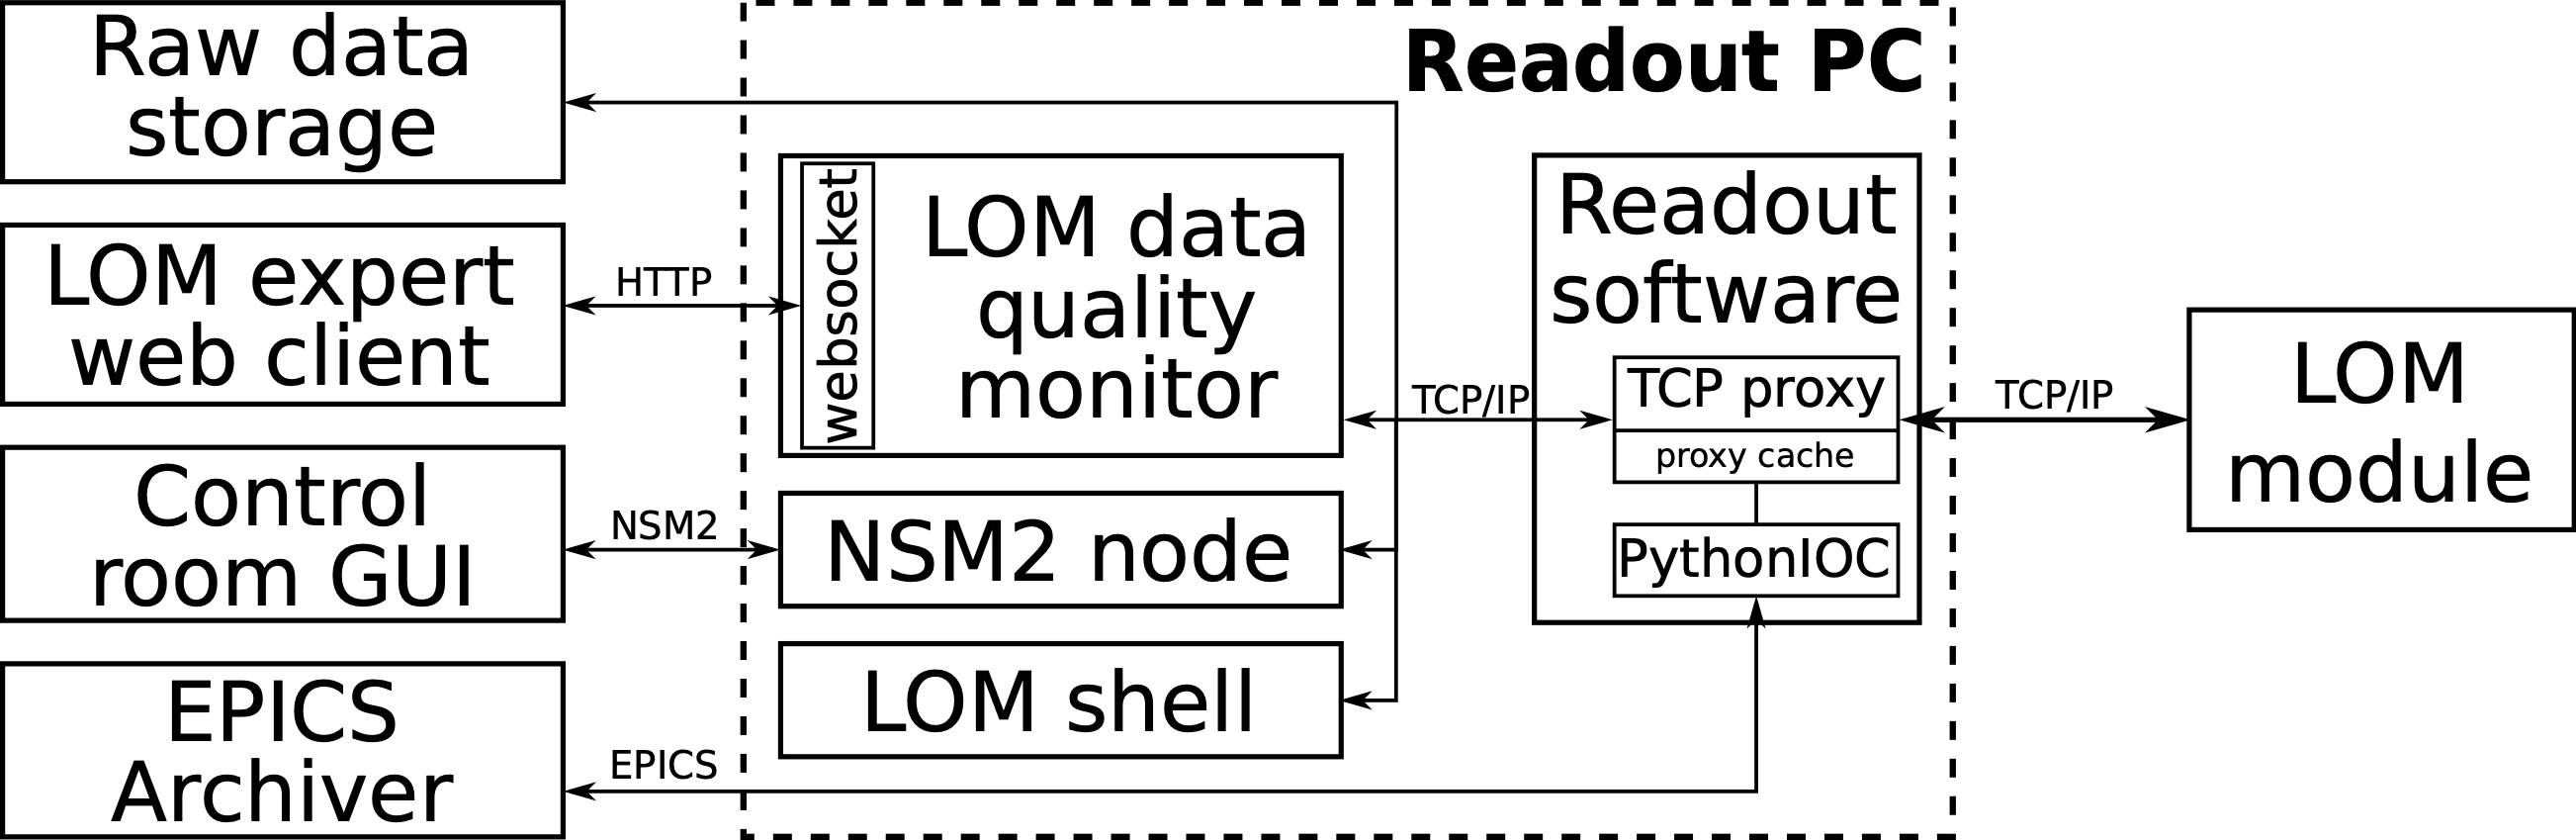
\includegraphics[width=\textwidth]{LOM_software.png}
\end{frame}

%TODO: ДОБАВИТЬ ГРАФИКИ СВЕТИМОСТЕЙ
\begin{frame}
\frametitle{Система медленного контроля EPICS}
    \begin{columns}
        \begin{column}{0.5\textwidth}
            \begin{itemize}
                \item Контроль набора данных
                \item Отслеживание корректности работы ускорителя
                \item Различные промежутки времени
                \item Создано 54 PV для значений светимостей/пьедесталов и других параметров с LOM
            \end{itemize}
        \end{column}
        \begin{column}{0.5\textwidth}
            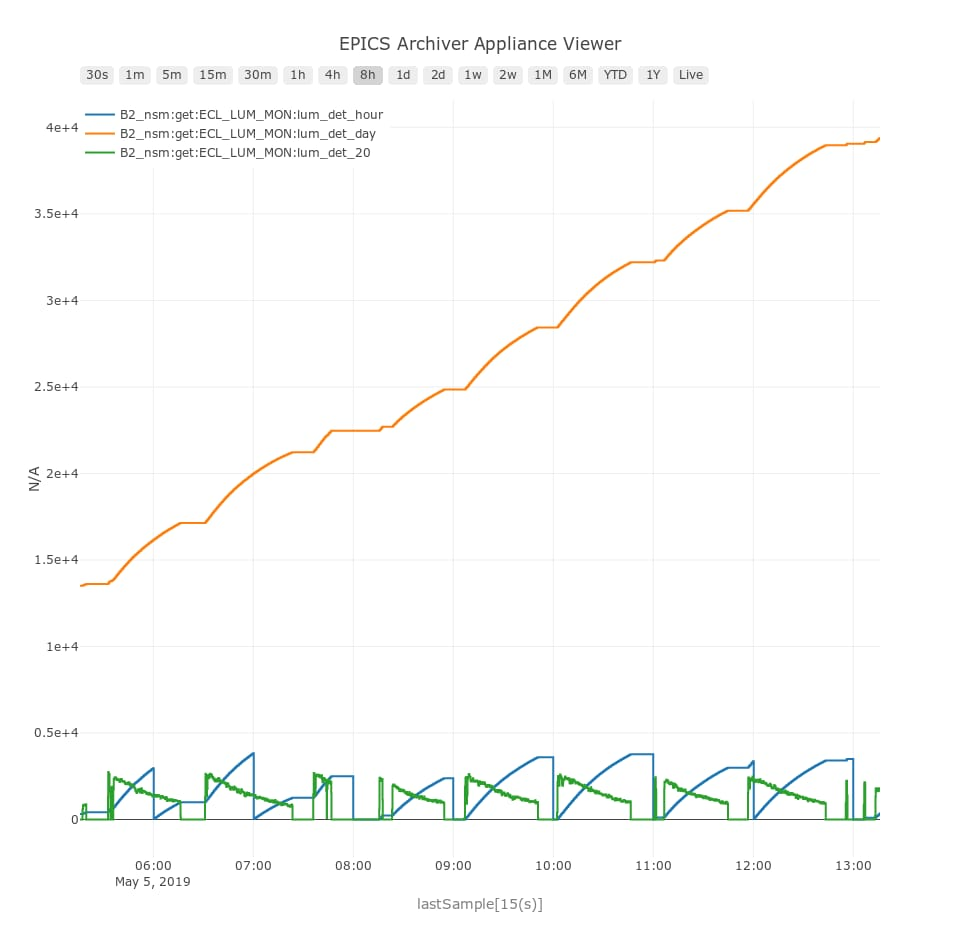
\includegraphics[width=\textwidth]{Int_lum.jpeg}
        \end{column}
    \end{columns}
\end{frame}


\begin{frame}
\frametitle{Отказоустойчивость ПО}
    Использовалась БД sqlite
    \begin{itemize}
        \item Сохранение значений светимости и дата последней модификации
        \item Сохранение значений светимости с предыдущих заходов
        \item Остановка чтения данных с монитора светимости при некорректных значениях заходов
    \end{itemize}
\end{frame}

\begin{frame}
\frametitle{Пьедесталы}
    \begin{itemize}
        \item Отслеживание работы калориметра
        \item Обнаружение зашумленных каналов
    \end{itemize}
    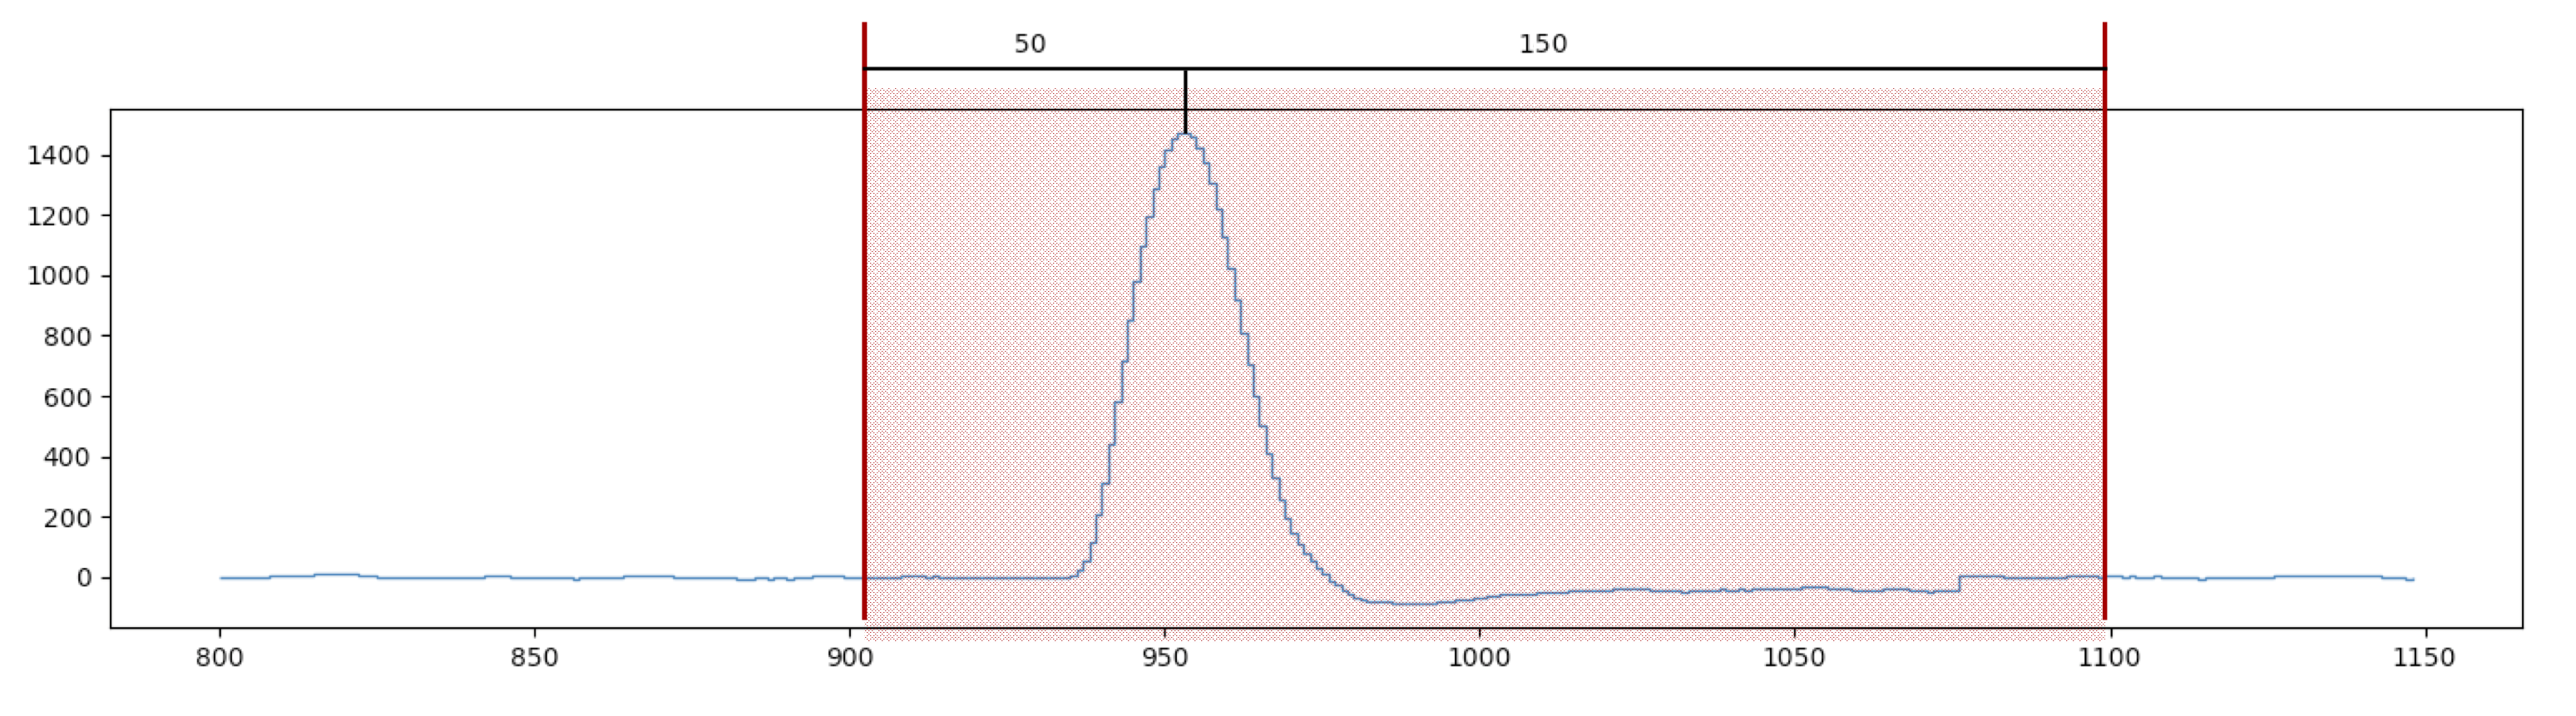
\includegraphics[width=\textwidth]{Pedestal.png}
\end{frame}

\begin{frame}
\frametitle{GUI}
    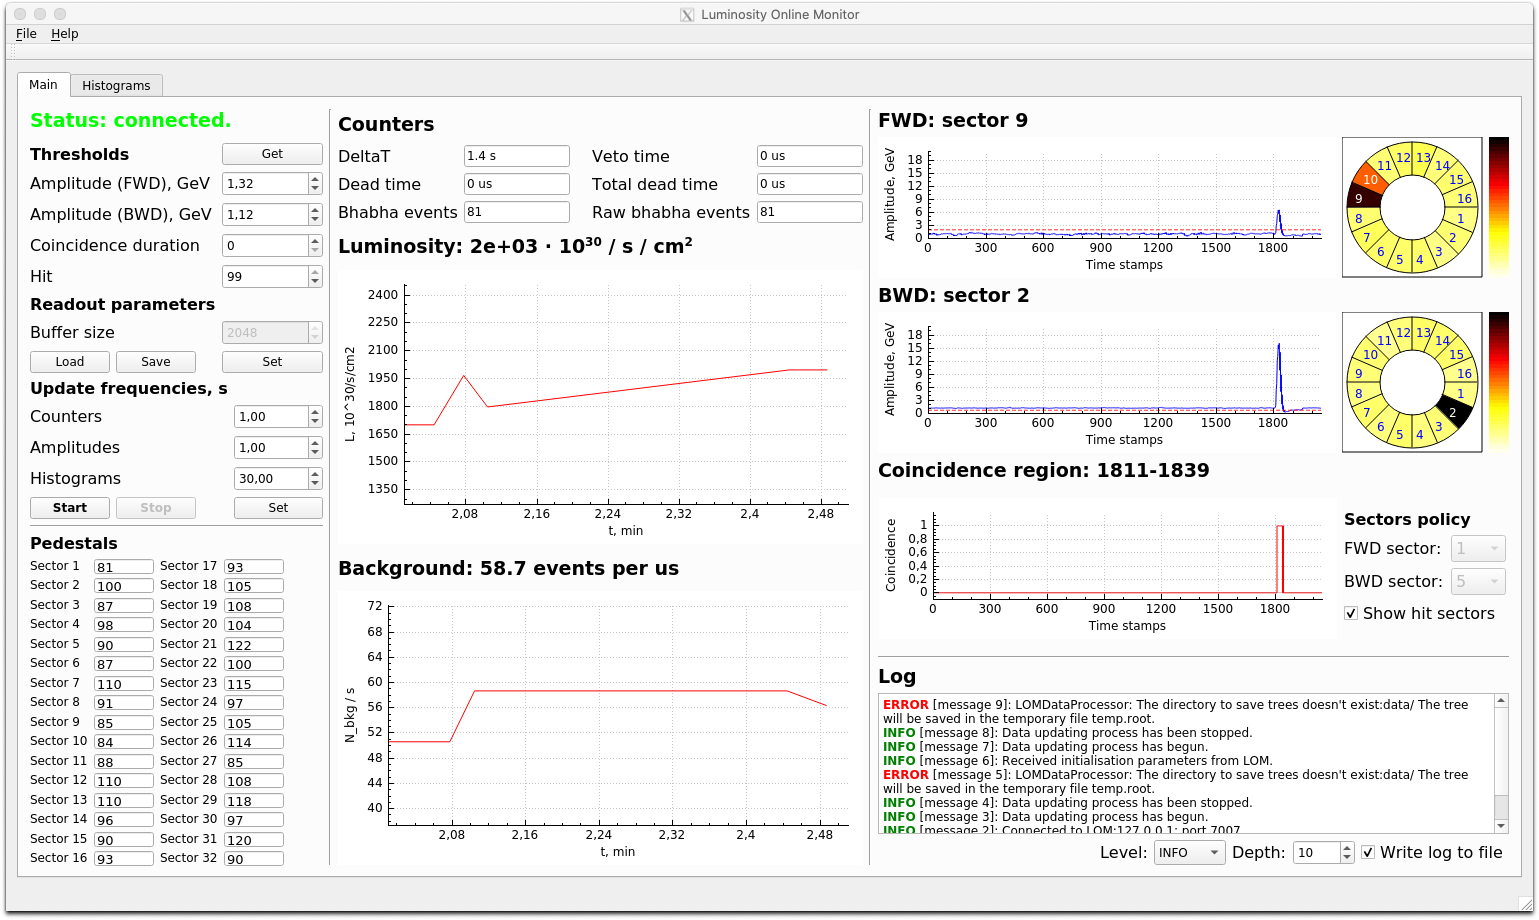
\includegraphics[width=\textwidth]{GUI3}
\end{frame}

\begin{frame}
\frametitle{Автоматизация калибровки LOM}
    \begin{itemize}
        \item Расширен протокол управления монитором светимости
        \item Реализована возможность параллельно устанавливать конфигурацию монитора и калориметра и управлять чтением данных с соответствующих модулей
        \item Калибровочные коэффициенты перенесены в БД
    \end{itemize}
\end{frame}

\begin{frame}
\frametitle{Заключение}
    \begin{itemize}
        \item Значительно расширено и оптимизировано ПО
        \item Добавлен расчет интегральных и максимальных светимостей, значений пьедесталов
        \item Доработано GUI для удаленной настройки параметров и отображения данных
        \item Усовершенствован процесс калибровки LOM
    \end{itemize}
\end{frame}

\end{document}

